\section{作业及答案：结构力学基础与技巧班第14次作业及答案（矩阵位移法）}
\begin{analysisbox}
矩阵位移法按单元刚度矩阵、坐标转换、整体刚度组装、边界条件处理和回代杆端力求解。编号清楚可显著减少代数错误。
\end{analysisbox}
\subsection*{第 1 页转写}
八、练习题

1.基本概念

8-1单元刚度矩阵是指下列两组量值之间关系的变换矩阵。（

）（北京科技大学

2010、中国地震局工程力学研究所2009、中南大学2010)

A.杆端位移和杆端力

B.杆端位移和结点位移

C.杆端位移和结点荷载

D.结点位移和结点荷载

8-2判断题。结构刚度矩阵反映了结构结点位移与荷载之间的关系。（

）（烟台

大学2013)

2.刚度矩阵的计算

8-3试用先处理法建立图8-43所示结构的结构刚度矩阵，忽略杆件的轴向变形

（EI=常数）。（湖南大学2008）

8-4求图8-44所示刚架结构刚度矩阵的任意两个主元素（自由结点）。已知各杆

I/A=1/10。（西南交通大学2010）

图8-43

图8-44

3.等效结点荷载

8-5图8-45所示结构按矩阵位移法计算，则与结点位移1、2（正方向见图虚线标

示）对应的等效结点荷载向量为

（浙江大学2012)

8-6图8-45所示结构，已知两杆EI=常数。若按矩阵位移法求得结点位移1、2分

别为91、$\triangle$2，则杆件BC左、右端的弯矩各为

（均以下侧受拉为正）。

（浙江大学2012）

8-7试求图8-46所示结构中结点3的综合结点荷载列阵F3=（X3Y3M3）T。

（中南大学2009）
\begin{figure}[H]\centering
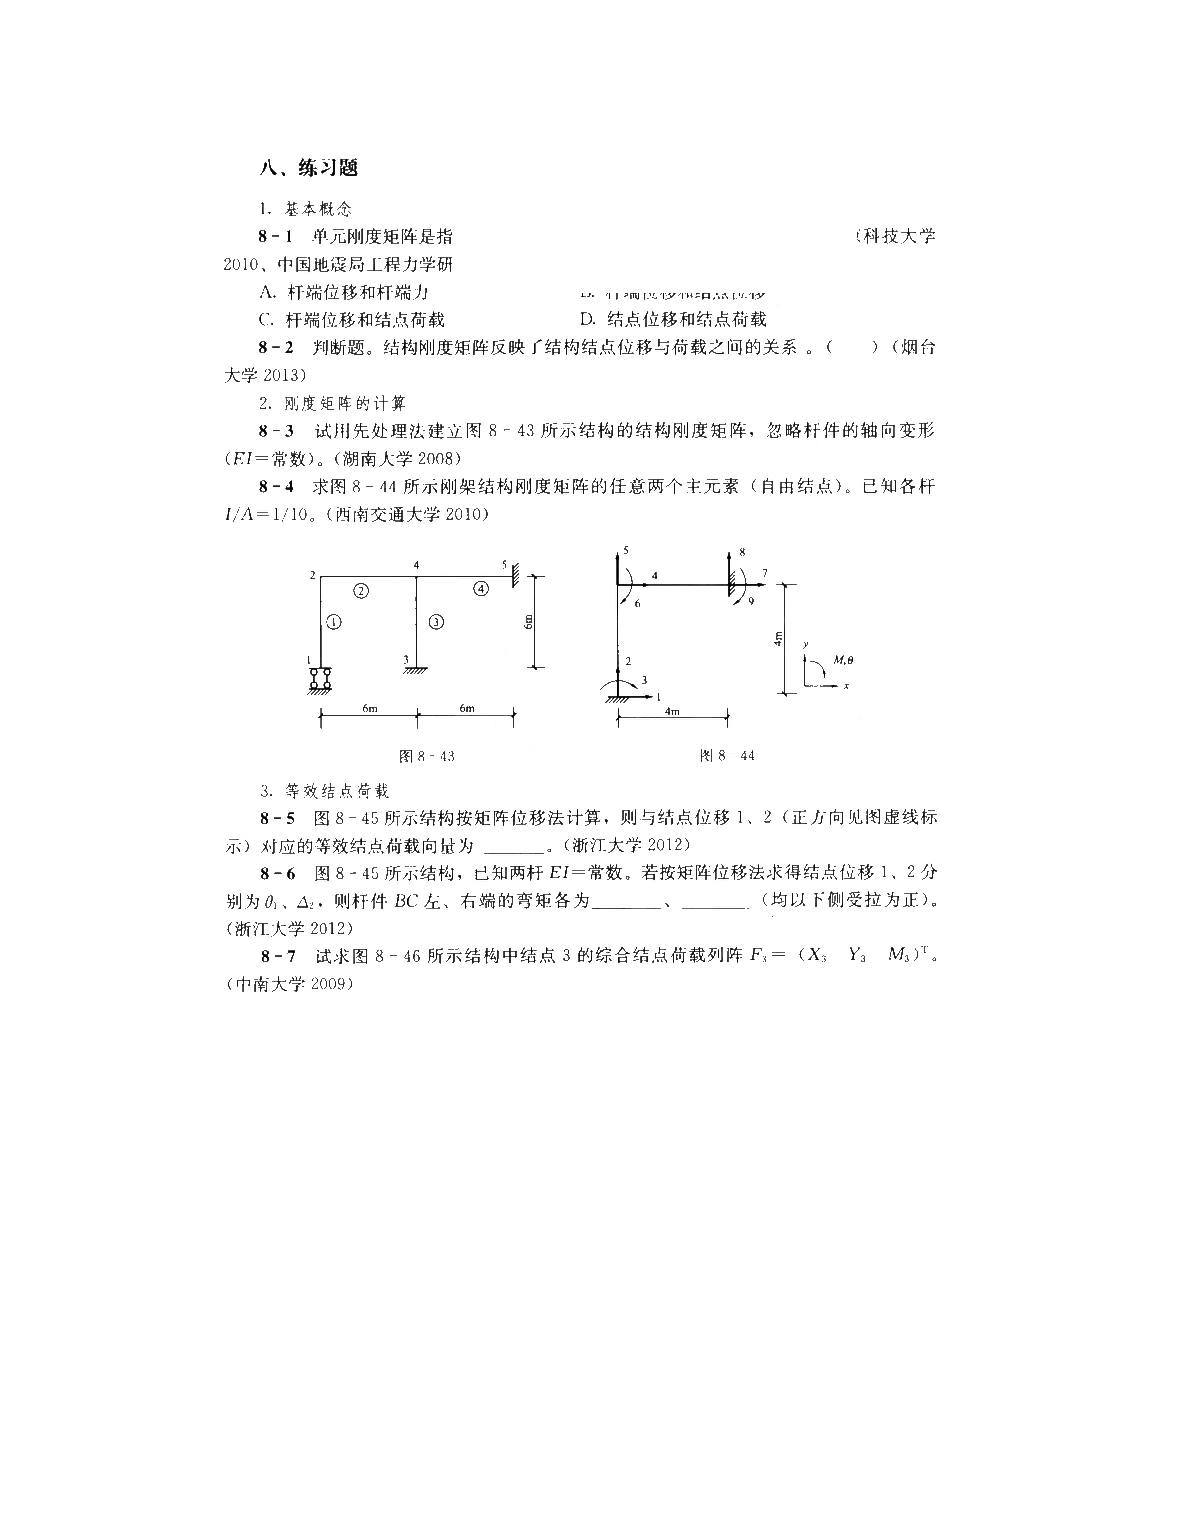
\includegraphics[width=0.92\textwidth]{figures/src17_p001.jpg}
\caption{结构力学基础与技巧班第14次作业及答案（矩阵位移法） 第 1 页清理图形页}
\end{figure}
\subsection*{第 2 页转写}
12kN/m

5kN-m

20kN

图8-45

图8-46

8-8按先处理法求图8-47所示连续梁的结点荷载列阵P。（西南交通大学2007）

8-9图8-48（a）所示结构，不考虑

轴向变形，整体坐标见图8-48（b），图中

20kN-m

(1,0,2)

括号内数码为结点总码（力和位移按水平、

(e0'1)

5kN

3kN

竖直、转动方向顺序排列），求等效结点荷载

列阵P。（山东建筑大学2008）

6kN/m

2kN

4kN

5kN-m

12kN/m

(0,0,0)

M,0

(0,0,0)

2EI

EI

EI

4m

(a)

(b)

图8-47

图8-48

8-10图8-49所示平面结构用矩阵位移法计算，引人支承条件后的整体刚度矩阵为

多少阶？求结点2和结点5的综合结点荷载列阵。（中南大学2011)

4.内力和位移的计算

8-11已知图8-50所示连续梁的结点

位移列阵4=（-0.0030.0040.005)T（分

别为结点2、3、4的转角），设各杆的E=2$\times$

10*kN/cm ，I=400cm，1=400cm。求单元

(2)的剪力和弯矩。（华南理工大学2010）

4kN-m

2.4kN/m

5.6kN-m

图8-49

图8-50

8-12采用矩阵位移法求图8-51所示桁架各杆轴力。已知：EA=60kN，Fp=100kN

（上海大学2008、武汉大学2008类似）

8-13图8-52所示结构，已知结点2的水平、竖向和转角位移分别为0、一0.0926、

一0.1667，结点3的转角为0.2220，试求23杆2端杆端力。已知单元刚度矩阵中的部分
\begin{figure}[H]\centering
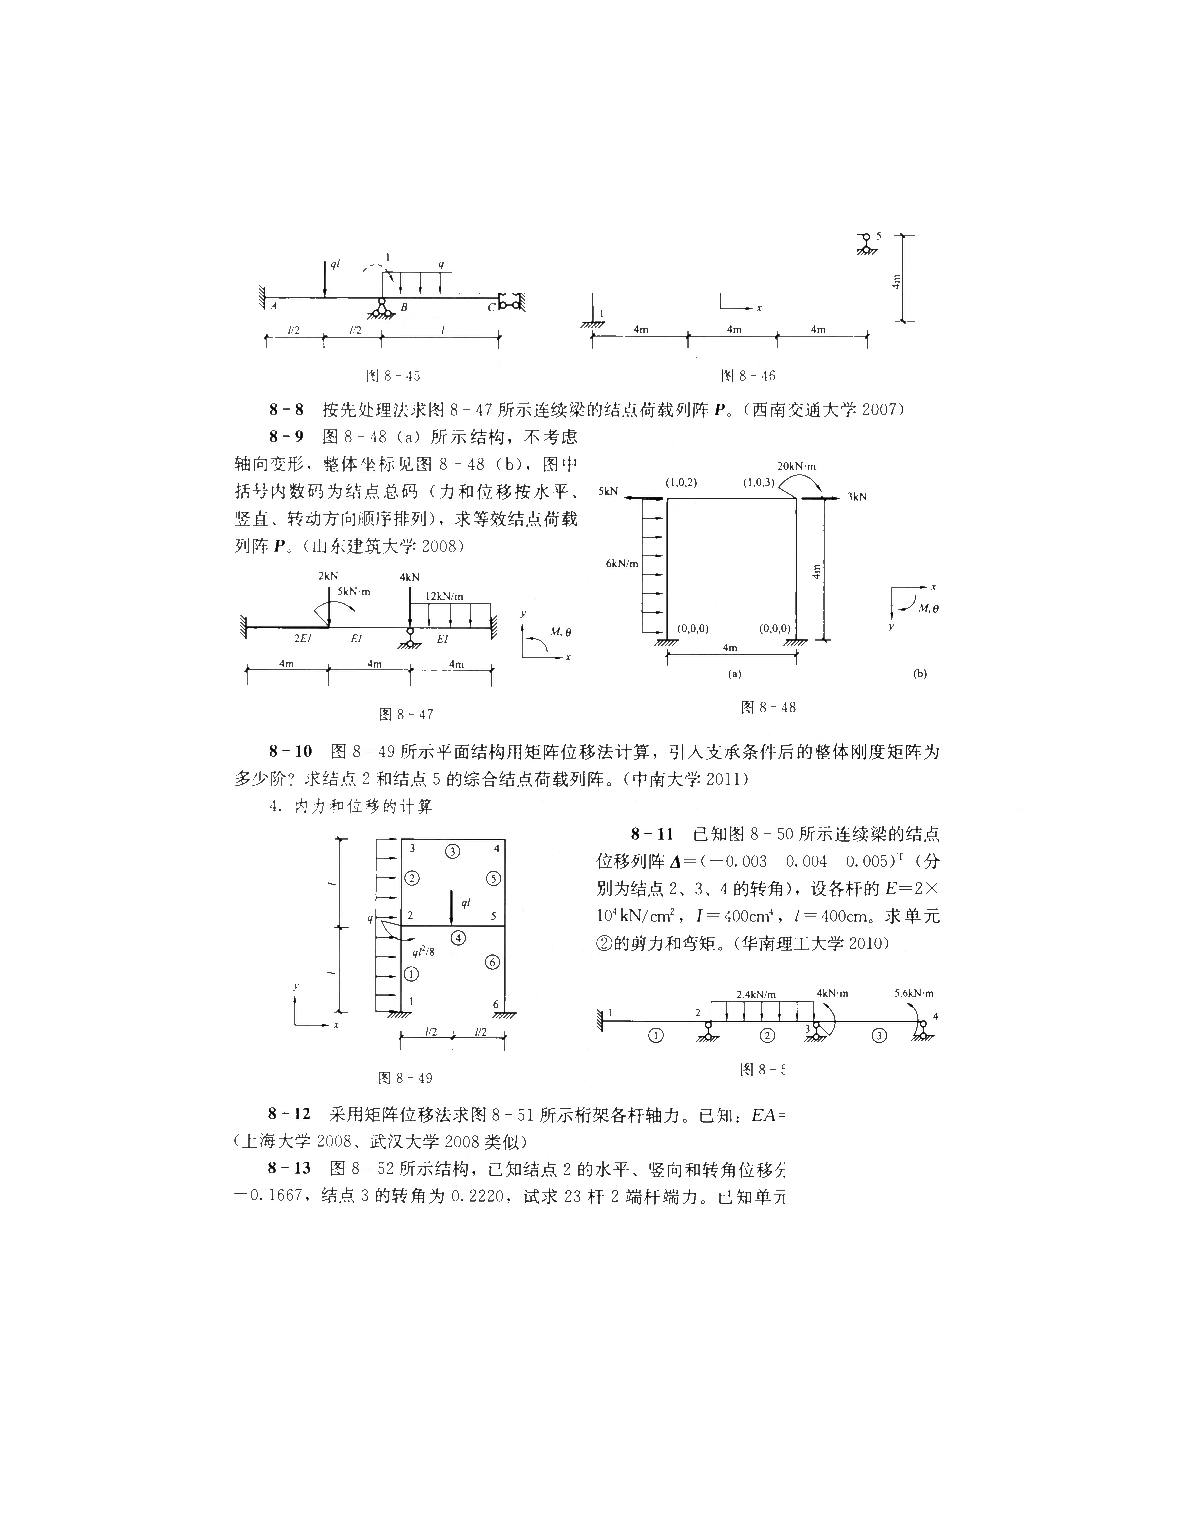
\includegraphics[width=0.92\textwidth]{figures/src17_p002.jpg}
\caption{结构力学基础与技巧班第14次作业及答案（矩阵位移法） 第 2 页清理图形页}
\end{figure}
\subsection*{第 3 页转写}
元素：

IkN

1kN-m

1o-2m

I-1m*

M,

4m

1m

图8-51

图8-52

12EI

6EI

4EI

k32=k62= ks3= kes

k33=2k63=k66

k22-

（浙江大

12

学2008)

8-14用矩阵位移法计算并作图8-53所示连续梁的弯矩图。各杆EI相同，为常数。

（重庆大学2009）

10kN/m

30kN-m

20kN

10kN

6m

6m

图8-53

九、练习题答案

8-1

A.

8-2

X。提示：反映的是结点位移和结点荷载之间的关系。

(EI/18

E1/6

8-3

K=

EI/6

4EI/3

EI/3。提示：建立顺时针坐标系。

EI/3

2EIJ

8-4K4=43EI/16，Kss=43EI/16，K66=2EI。注意：（1）本题为逆时针坐标系，

变。（2）竖杆单元需要坐标变换，若假设单元方向向上，则$\alpha$=90$^\circ$。

8-5

 ql /24;ql/2。

4EI01\_6EIA2

2EI+6EI2\_?

8-6

12

12

12

12

F3=（0-34kN

8-7

一9kN m)T（假设杆端弯矩逆时针为正）。

8-8

P=Pe+Pp=(0

-16)T+(-2-50)T=(-2kN-5kN-16kN m)T。

注意：题中4kN的结点力作用在支座处，对结点荷载列阵无影响。

P=Pe+Pp=（12

8-9

-80)T+（-5+3020)T=(10kN-8kN m

20kNm)"。
\begin{figure}[H]\centering
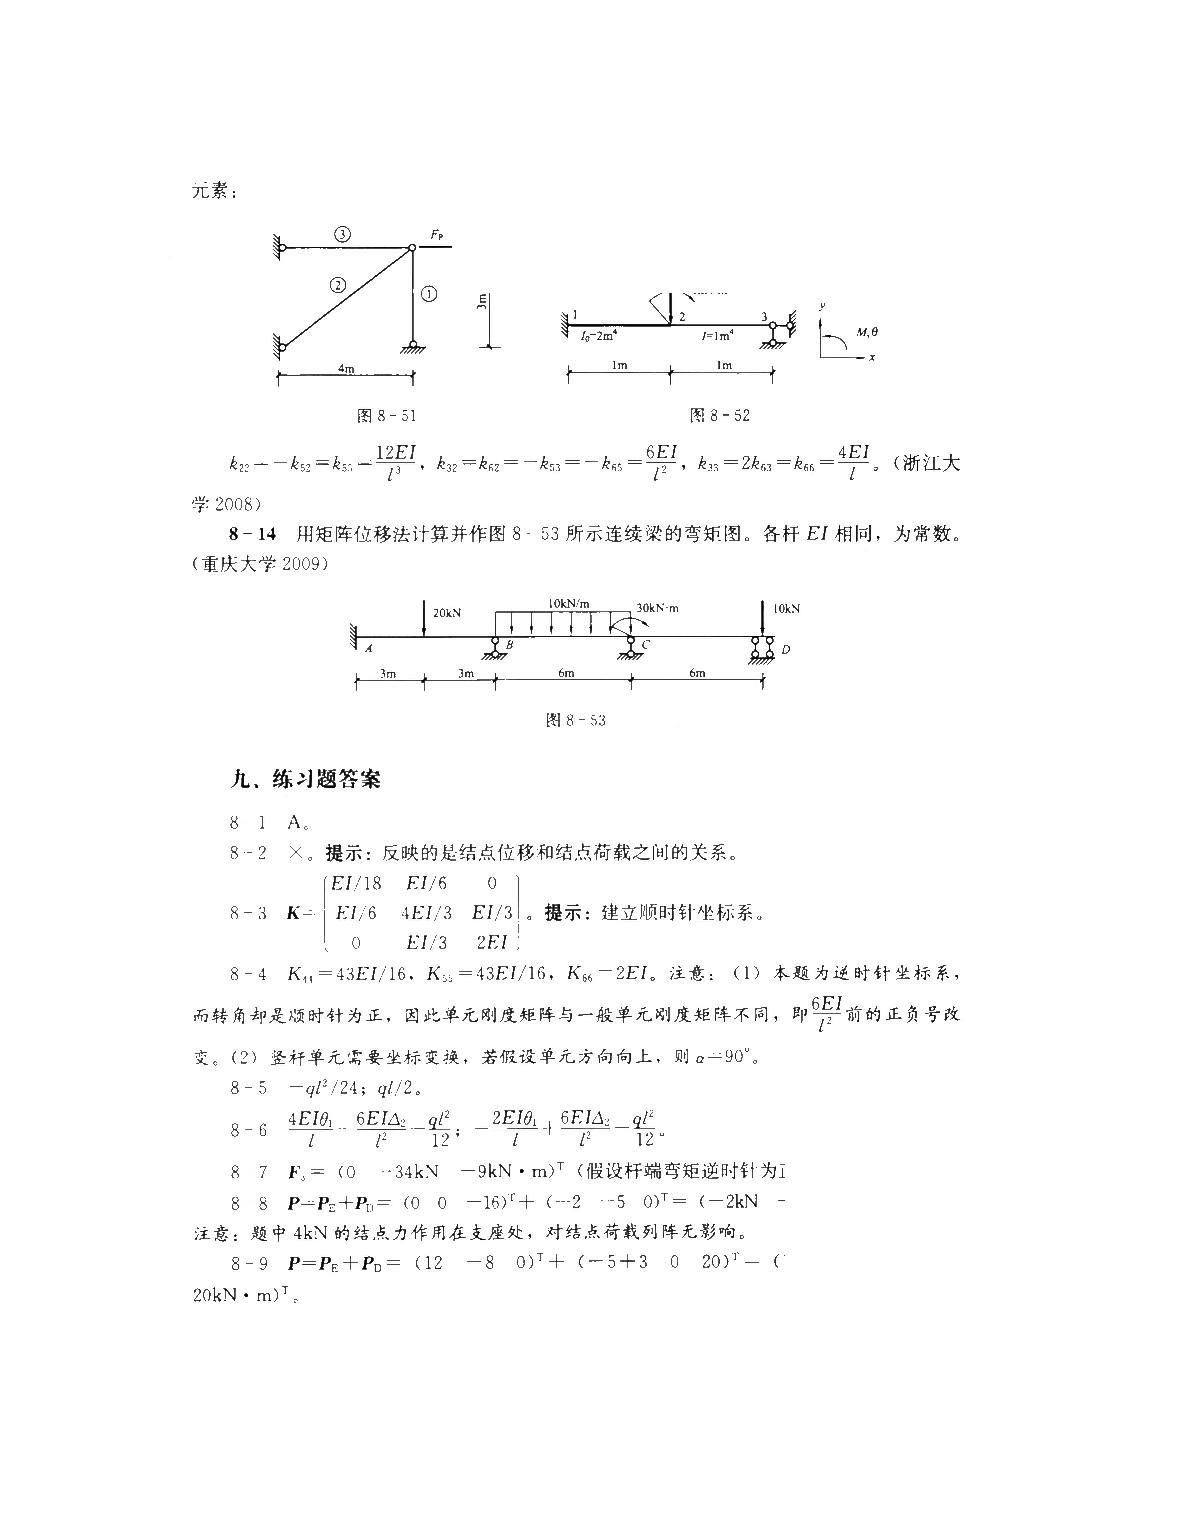
\includegraphics[width=0.92\textwidth]{figures/src17_p003.jpg}
\caption{结构力学基础与技巧班第14次作业及答案（矩阵位移法） 第 3 页清理图形页}
\end{figure}
\subsection*{第 4 页转写}
8-1012阶。P2=（ql ql/20)T，Ps=（0 ql/2q /8)T（假设杆端弯矩逆

时针为正)。

5. 1kN

2.4kN m

8-11

FO-

提示：原题未规定结点转角的正方向，读者可以根据荷

4.5kN

-1.2kN m)

载情况判断出4结点转角应该为逆时针，而已知条件中4结点的转角为0.005（正值），由

此可推知逆时针为正。建立图8-54所示坐标系。

8-12各杆轴力见图8-55。

8-13

（0-0.7794E-0.7784E)。提示：用公式Fe=k。题中未给出单元刚度

矩阵中的第一行元素，需要读者自行记住。

8-14

M图见图8-56。

70.37

22.22

32

23

11

M,6

13

FN(单位：kN)

M图(单位：kN-m)

图8-55

图8-54

图8-56
\begin{figure}[H]\centering
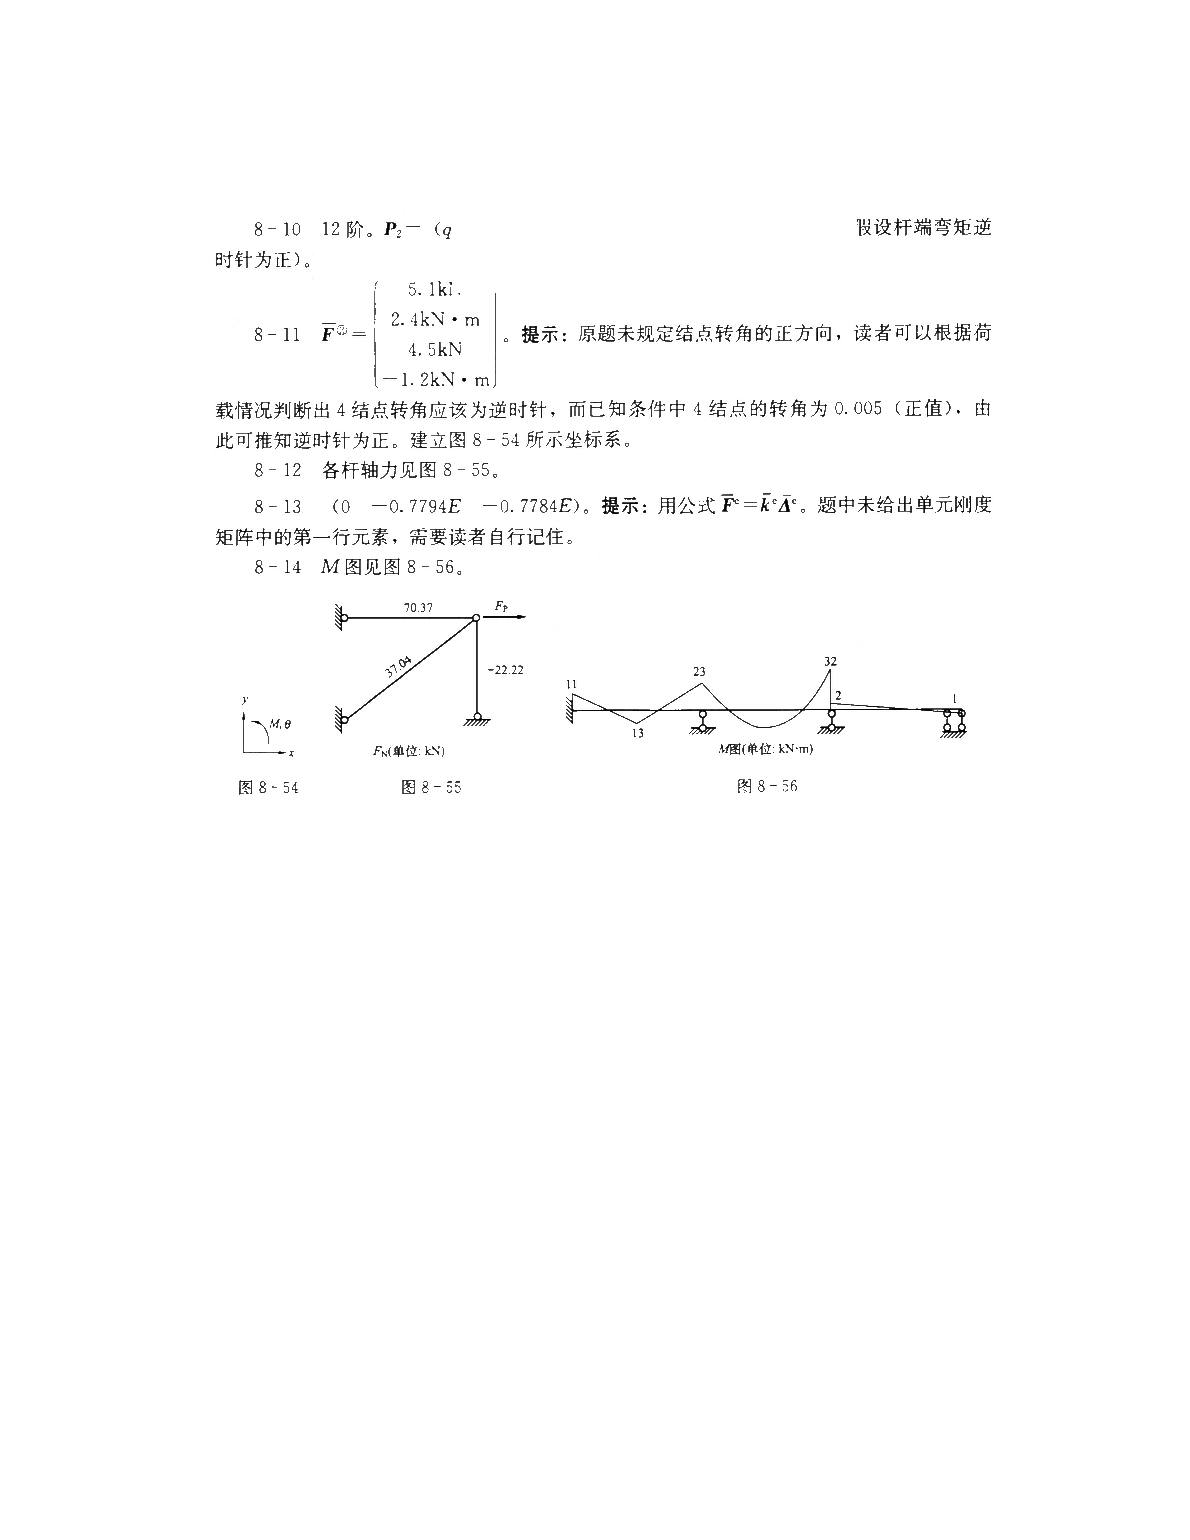
\includegraphics[width=0.92\textwidth]{figures/src17_p004.jpg}
\caption{结构力学基础与技巧班第14次作业及答案（矩阵位移法） 第 4 页清理图形页}
\end{figure}
